%!TEX root = thesis.tex
%% %% ***************** Results *****************


\section{Results}\label{sec:results}

We start this section by looking at
the Azure resources needed for ML training
both in general Azure environment and in ML Studio.
Next we analyze the results of
different ML algorithms and pipelines.

%% ************************************************************************************************************

\subsection{Azure and Azure ML Studio}\label{subsec:res-azure-and-azure-ml-studio}

\subsubsection*{Azure resources}

As stated in section~\ref{subsec:meth-azure-environment},
Azure provides a vast set of tools and resources
for different kinds of cloud projects.
Resources needed for Azure ML Studio usage
depends on the subscription used
and security restrictions set by subscription administrators.
When starting this study,
due to these restrictions,
all resources used for ML training in this project
needed to be inside the same virtual network.
Azure ML Studio environment could be opened from any network,
but most of the features were unavailable
if computer browsing studio UI was outside this virtual network.
Thus,
a virtual machine had to be acquired as Azure resource
from within the same network as other resources
and ML Studio UI had to be opened with the browser on this machine.
Later on it was found
that Azure Machine Learning Workspace networking feature
could be configured to allow public access
making possible to access ML Studio UI from all networks.


%% TODO: add picture to explain this

%% ............................................................................................................

\subsubsection*{Azure ML Studio components}

During the initial pipeline runs
the execution came to an abrupt stop
and Azure notified about memory issues.
These problems were linked to the data amount
which had to be reduced to 600 megabytes
before any pipeline could be finished using the data.
This reduction was against the initial goal
where preferably all the data could have been used.

Considerable amount of time was used
to fix or avoid this issue
but nothing clear was found
that would explain the error received.
While working with the issue
it was also noted
that data needed more cleaning
in order to ease the preprocessing phase
as described with more detail in section~\ref{subsec:meth-data-anonymization}
Thus,
the data had to be imported from log archive
and anonymized once more.

To advance the study more efficiently
it was decided to trim info-type log messages from data
hence reducing the data amount considerably.
Final data included 8.6 million log rows
which was about 10\% of the original data size.
Before final cleaning operations
the data took 8.1GB od disk space,
and after cleaning the rawmessage-field
the final disk size was 6.6GB.
Even with this data size,
some Azure ML components faced this memory issue
and forced us to choose such components
that were able to handle these data amounts.

%% TODO: Move some parts of the above memory problem elsewhere

In addition to the data we used to train the algorithm,
we needed to set up computing instance
in Azure ML studio.
Some predefined resource limitations
affected the computing instance choosing
and the memory issue encouraged us
to pick memory prioritized instances.
Single computing instance did not work,
but we needed to choose a computing cluster instead
to be able to run ML training pipeline.
%% TODO: Maybe what other choises were possible?

%% TODO: Data stores etc?


%% ************************************************************************************************************


\subsection{ML training and validation}\label{subsec:res-ml-training-and-validation}

In the methods section~\ref{subsec:meth-ml-pipeline}
we discussed of different approaches that could be used
to get the best results from the ML training.
In order to compare different results,
some comparable metrics are needed.
%% TODO: declare comparable metrics etc.

%% TODO: move to methods-section???
Several crossing points caused the pipeline to diverge.
First,
the error message used to calculate the anomaly probability of a log row
had two options.
We could either use simple \textit{message},
or more verbose \textit{rawmessage}.
This textual data could be fed to the ADA-component in several forms.
Most straightforward way was using textual data without any preformatting.
Text could also be run through \enquote{Preprocess text} -component. %% TODO: Explain somewhere!
N-gram features could have been extracted from the text
and these features could have been used instead.
Instead of n-gram features,
textual data could be converted to numeric
with \enquote{Feature Hashing} -component.
After getting the ADA-component results,
the anomaly probabilities were compressed with R-code or SQL. %% TODO: ?
<This concludes the phase 1.> %% TODO: ??

In phase two,
diverging of the pipeline was due to either different regression algorithms used
or result comparison to disregarding the results of phase 1.
In practice this means
that in order to validate the results against our initial hypothesis,
we used statistical log data such as row count and unique job ID count
without anomaly probabilities
to determine whether anomaly metrics provided any insight regarding the ticket data.

Each diverging step, or layer,
multiplies the amount of results used in final comparison
that would determine the best possible pipeline combination.
These layers are simplified in the table~\ref{tab:ml-pipeline-diverging}.

\begin{table}[]
    \begin{tabular}{|l|l|l|}
        \hline
        \textbf{Divergent layer}           & \textbf{Options}                                                              & \textbf{Divergent count} \\ \hline
        Input text column                  & \begin{tabular}[c]{@{}l@{}}message \\ rawmessage\end{tabular}                 & 2                        \\ \hline
        Text preprocess                    & \begin{tabular}[c]{@{}l@{}}Yes\\ No\end{tabular}                              & 2                        \\ \hline
        Numeric conversion                 & \begin{tabular}[c]{@{}l@{}}No\\ N-gram Feature\\ Feature Hashing\end{tabular} & 3                        \\ \hline
        ADA training                       & \begin{tabular}[c]{@{}l@{}}Unconventional \\ Proper\end{tabular}              & 2                        \\ \hline
        Validation without anomaly metrics & \begin{tabular}[c]{@{}l@{}}Yes\\ No\end{tabular}                           & 2                        \\ \hline
        Regression algorithms &
        \begin{tabular}[c]{@{}l@{}}Decision forest regression \\ Boosted decision tree regression \\ Neural Network Regression \\ Linear regression\end{tabular} &
        4 \\ \hline
    \end{tabular}
    \caption{Pipeline divergent layers}
    \label{tab:ml-pipeline-diverging}
\end{table}

The divergent count implies the number of branches
diverging from the previous component.
The total count of branch ends, or leaves,
would then be the multiplication of all divergent counts,
totaling to 192 comparable pipeline combinations.
Moreover,
n-gram feature extraction and feature hashing
have several tunable parameters
that strongly influence the end results of the algorithm training.
To reduce this amount when considering the best possible pipeline,
we simplified this by narrowing down the options 
based on initial test run results of some of the divergent options.

For example, 
n-gram feature component suffered greatly from the memory problem %% TODO: refer to it?
and the data amount that the \textit{Extract N-Gram Features from Text} -component
was able to handle only 2\% of the original data amount.
This was deemed as too small amount for training
as it would be extremely likely with 98\% of the data skipped
that also possible rows relevant to the ticket anomalies
would get trimmed out.


%% ************************************************************************************************************

\clearpage

\toimhuom{Next is some initial values from pipeline runs. Subjected to change!}

\subsubsection*{N-Gram feature extraction}
Using Decision forest regression algorithm.
\\
\begin{figure}[htb]
    \centering
    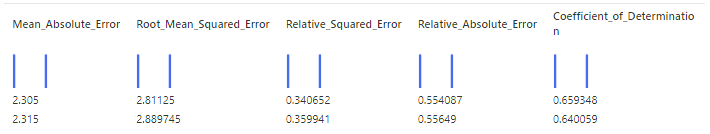
\includegraphics[width=150mm]{./appendices/msg_ngram_decision-forest-reg_lewd2unanom.png}
    \caption{Message with N-Gram feature extraction
    using unconventional training method in phase 1,
        Decision forest regression in phase 2,
        compared to method without anomaly values.
        \label{fig:msg_ngram_decision-forest-reg_lewd2unanom}}
\end{figure}

\begin{figure}[htb]
    \centering
    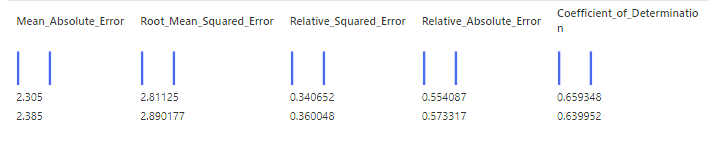
\includegraphics[width=150mm]{./appendices/msg_ngram_decision-forest-reg_proper2unanom.png}
    \caption{Message with N-Gram feature extraction
    using proper training method in phase 1,
        Decision forest regression in phase 2,
        compared to method without anomaly values.
        \label{fig:msg_ngram_decision-forest-reg_proper2unanom}}
\end{figure}

\begin{figure}[htb]
    \centering
    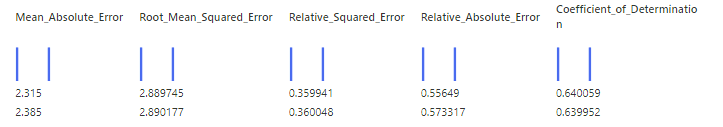
\includegraphics[width=150mm]{./appendices/msg_ngram_decision-forest-reg_lewd2proper.png}
    \caption{Message with N-Gram feature extraction
    using Decision forest regression in phase 2,
        comparing unconventional training to proper training.
        \label{fig:msg_ngram_decision-forest-reg_lewd2proper}}
\end{figure}



\clearpage

%% ............................................................................................................

\subsubsection*{Anomaly detection with pure textual data}

\begin{figure}[htb]
    \centering
    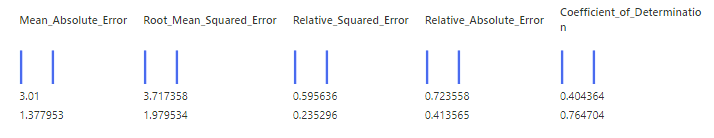
\includegraphics[width=150mm]{./appendices/msg_pure_decision-forest-reg_lewd2unanom.png}
    \caption{Message fed pure to ADA-component,
    using unconventional training method in phase 1,
        Decision forest regression in phase 2,
        compared to method without anomaly values.
        \label{fig:msg_pure_decision-forest-reg_lewd2unanom}}
\end{figure}

\begin{figure}[htb]
    \centering
    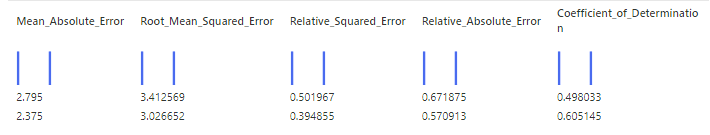
\includegraphics[width=150mm]{./appendices/msg_pure_decision-forest-reg_proper2unanom.png}
    \caption{Message fed pure to ADA-component,
        using proper training method in phase 1,
        Decision forest regression in phase 2,
        compared to method without anomaly values.
        \label{fig:msg_pure_decision-forest-reg_proper2unanom}}
\end{figure}



\begin{figure}[htb]
    \centering
    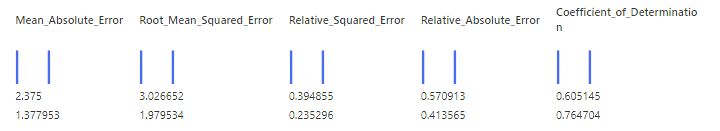
\includegraphics[width=150mm]{./appendices/msg_pure_decision-forest-reg_lewd2proper.png}
    \caption{Message fed pure to ADA-component,
    using Decision forest regression in phase 2,
        comparing unconventional training to proper training.
        \label{fig:msg_pure_decision-forest-reg_lewd2proper}}
\end{figure}

\clearpage